% 1977 年陕西卷第十题图 1：正方形 ABCD 的角 B 处切着两边截去半径为 r 的圆料，
% 截出的正方形 A′B′C′D 与原正方形共角 D，顶点 B′ 落在对角线 BD 与圆的交点处（按源卷第 5 页布局）
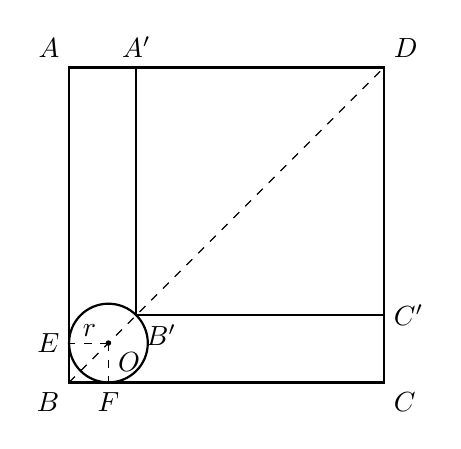
\begin{tikzpicture}[scale=1.0]
  \draw[thick] (0,0)--(4,0)--(4,4)--(0,4)--cycle;
  \draw[thick] (0.8536,4)--(0.8536,0.8536);
  \draw[thick] (0.8536,0.8536)--(4,0.8536);
  \draw[thick] (0.5,0.5) circle (0.5);
  \draw[dashed] (0,0)--(4,4);
  \draw[dashed] (0.5,0.5)--(0,0.5);
  \draw[dashed] (0.5,0.5)--(0.5,0);
  \fill (0.5,0.5) circle (1pt) node[below right] {$O$};
  \node at (0.26,0.66) {$r$};
  \node[left]  at (0,0.5)   {$E$};
  \node[below] at (0.5,0)   {$F$};
  \node[above left]  at (0,4)      {$A$};
  \node[above]       at (0.8536,4) {$A'$};
  \node[above right] at (4,4)      {$D$};
  \node[right]  at (4,0.8536) {$C'$};
  \node[below right] at (4,0)      {$C$};
  \node[below left]  at (0,0)      {$B$};
  \node[below right] at (0.8536,0.8536) {$B'$};
\end{tikzpicture}
